\documentclass[1p]{elsarticle_modified}
%\bibliographystyle{elsarticle-num}

%\usepackage[colorlinks]{hyperref}
%\usepackage{abbrmath_seonhwa} %\Abb, \Ascr, \Acal ,\Abf, \Afrak
\usepackage{amsfonts}
\usepackage{amssymb}
\usepackage{amsmath}
\usepackage{amsthm}
\usepackage{scalefnt}
\usepackage{amsbsy}
\usepackage{kotex}
\usepackage{caption}
\usepackage{subfig}
\usepackage{color}
\usepackage{graphicx}
\usepackage{xcolor} %% white, black, red, green, blue, cyan, magenta, yellow
\usepackage{float}
\usepackage{setspace}
\usepackage{hyperref}

\usepackage{tikz}
\usetikzlibrary{arrows}

\usepackage{multirow}
\usepackage{array} % fixed length table
\usepackage{hhline}

%%%%%%%%%%%%%%%%%%%%%
\makeatletter
\renewcommand*\env@matrix[1][\arraystretch]{%
	\edef\arraystretch{#1}%
	\hskip -\arraycolsep
	\let\@ifnextchar\new@ifnextchar
	\array{*\c@MaxMatrixCols c}}
\makeatother %https://tex.stackexchange.com/questions/14071/how-can-i-increase-the-line-spacing-in-a-matrix
%%%%%%%%%%%%%%%

\usepackage[normalem]{ulem}

\newcommand{\msout}[1]{\ifmmode\text{\sout{\ensuremath{#1}}}\else\sout{#1}\fi}
%SOURCE: \msout is \stkout macro in https://tex.stackexchange.com/questions/20609/strikeout-in-math-mode

\newcommand{\cancel}[1]{
	\ifmmode
	{\color{red}\msout{#1}}
	\else
	{\color{red}\sout{#1}}
	\fi
}

\newcommand{\add}[1]{
	{\color{blue}\uwave{#1}}
}

\newcommand{\replace}[2]{
	\ifmmode
	{\color{red}\msout{#1}}{\color{blue}\uwave{#2}}
	\else
	{\color{red}\sout{#1}}{\color{blue}\uwave{#2}}
	\fi
}

\newcommand{\Sol}{\mathcal{S}} %segment
\newcommand{\D}{D} %diagram
\newcommand{\A}{\mathcal{A}} %arc


%%%%%%%%%%%%%%%%%%%%%%%%%%%%%5 test

\def\sl{\operatorname{\textup{SL}}(2,\Cbb)}
\def\psl{\operatorname{\textup{PSL}}(2,\Cbb)}
\def\quan{\mkern 1mu \triangleright \mkern 1mu}

\theoremstyle{definition}
\newtheorem{thm}{Theorem}[section]
\newtheorem{prop}[thm]{Proposition}
\newtheorem{lem}[thm]{Lemma}
\newtheorem{ques}[thm]{Question}
\newtheorem{cor}[thm]{Corollary}
\newtheorem{defn}[thm]{Definition}
\newtheorem{exam}[thm]{Example}
\newtheorem{rmk}[thm]{Remark}
\newtheorem{alg}[thm]{Algorithm}

\newcommand{\I}{\sqrt{-1}}
\begin{document}

%\begin{frontmatter}
%
%\title{Boundary parabolic representations of knots up to 8 crossings}
%
%%% Group authors per affiliation:
%\author{Yunhi Cho} 
%\address{Department of Mathematics, University of Seoul, Seoul, Korea}
%\ead{yhcho@uos.ac.kr}
%
%
%\author{Seonhwa Kim} %\fnref{s_kim}}
%\address{Center for Geometry and Physics, Institute for Basic Science, Pohang, 37673, Korea}
%\ead{ryeona17@ibs.re.kr}
%
%\author{Hyuk Kim}
%\address{Department of Mathematical Sciences, Seoul National University, Seoul 08826, Korea}
%\ead{hyukkim@snu.ac.kr}
%
%\author{Seokbeom Yoon}
%\address{Department of Mathematical Sciences, Seoul National University, Seoul, 08826,  Korea}
%\ead{sbyoon15@snu.ac.kr}
%
%\begin{abstract}
%We find all boundary parabolic representation of knots up to 8 crossings.
%
%\end{abstract}
%\begin{keyword}
%    \MSC[2010] 57M25 
%\end{keyword}
%
%\end{frontmatter}

%\linenumbers
%\tableofcontents
%
\newcommand\colored[1]{\textcolor{white}{\rule[-0.35ex]{0.8em}{1.4ex}}\kern-0.8em\color{red} #1}%
%\newcommand\colored[1]{\textcolor{white}{ #1}\kern-2.17ex	\textcolor{white}{ #1}\kern-1.81ex	\textcolor{white}{ #1}\kern-2.15ex\color{red}#1	}

{\Large $\underline{12a_{0085}~(K12a_{0085})}$}

\setlength{\tabcolsep}{10pt}
\renewcommand{\arraystretch}{1.6}
\vspace{1cm}\begin{tabular}{m{100pt}>{\centering\arraybackslash}m{274pt}}
\multirow{5}{120pt}{
	\centering
	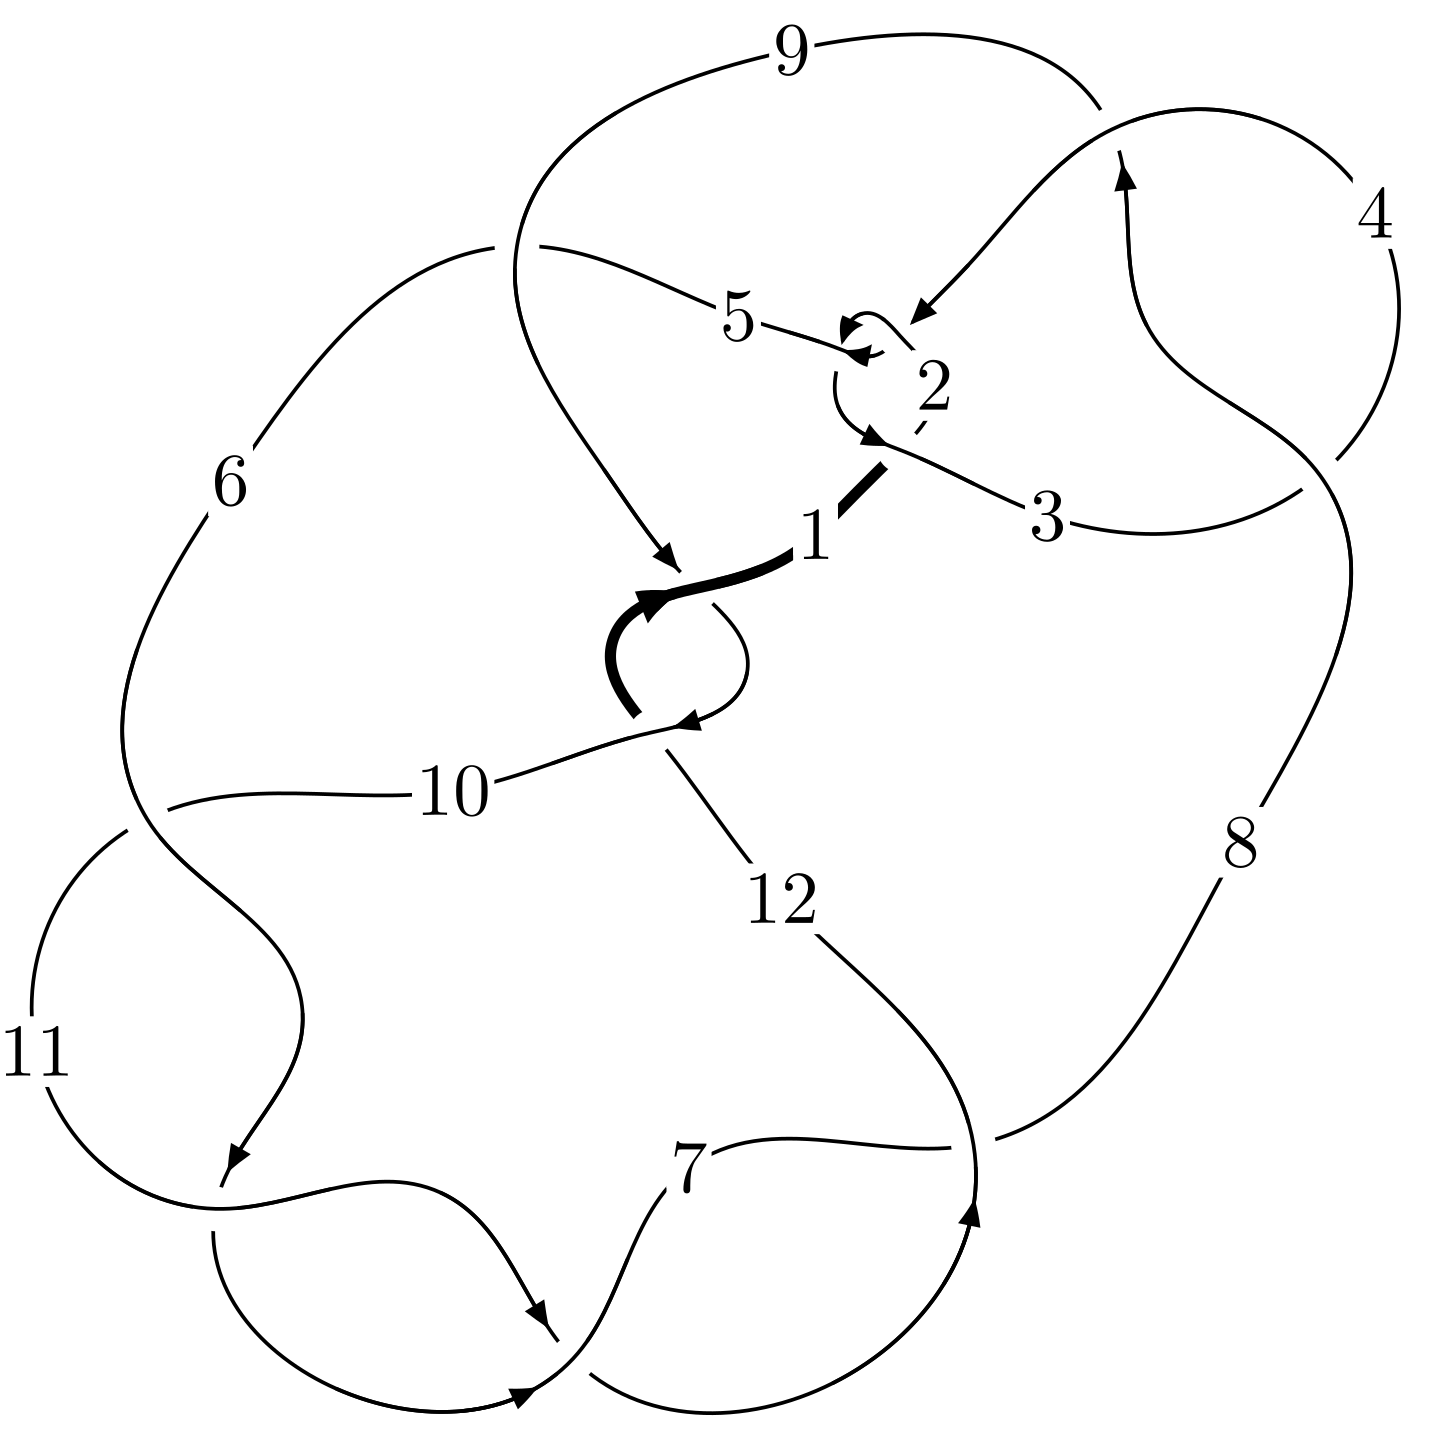
\includegraphics[width=112pt]{../../../GIT/diagram.site/Diagrams/png/886_12a_0085.png}\\
\ \ \ A knot diagram\footnotemark}&
\allowdisplaybreaks
\textbf{Linearized knot diagam} \\
\cline{2-2}
 &
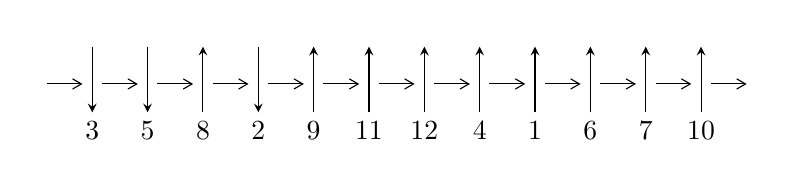
\begin{tikzpicture}[x=20pt, y=17pt]
	% nodes
	\node (C0) at (0, 0) {};
	\node (C1) at (1, 0) {};
	\node (C1U) at (1, +1) {};
	\node (C1D) at (1, -1) {3};

	\node (C2) at (2, 0) {};
	\node (C2U) at (2, +1) {};
	\node (C2D) at (2, -1) {5};

	\node (C3) at (3, 0) {};
	\node (C3U) at (3, +1) {};
	\node (C3D) at (3, -1) {8};

	\node (C4) at (4, 0) {};
	\node (C4U) at (4, +1) {};
	\node (C4D) at (4, -1) {2};

	\node (C5) at (5, 0) {};
	\node (C5U) at (5, +1) {};
	\node (C5D) at (5, -1) {9};

	\node (C6) at (6, 0) {};
	\node (C6U) at (6, +1) {};
	\node (C6D) at (6, -1) {11};

	\node (C7) at (7, 0) {};
	\node (C7U) at (7, +1) {};
	\node (C7D) at (7, -1) {12};

	\node (C8) at (8, 0) {};
	\node (C8U) at (8, +1) {};
	\node (C8D) at (8, -1) {4};

	\node (C9) at (9, 0) {};
	\node (C9U) at (9, +1) {};
	\node (C9D) at (9, -1) {1};

	\node (C10) at (10, 0) {};
	\node (C10U) at (10, +1) {};
	\node (C10D) at (10, -1) {6};

	\node (C11) at (11, 0) {};
	\node (C11U) at (11, +1) {};
	\node (C11D) at (11, -1) {7};

	\node (C12) at (12, 0) {};
	\node (C12U) at (12, +1) {};
	\node (C12D) at (12, -1) {10};
	\node (C13) at (13, 0) {};

	% arrows
	\draw[->,>={angle 60}]
	(C0) edge (C1) (C1) edge (C2) (C2) edge (C3) (C3) edge (C4) (C4) edge (C5) (C5) edge (C6) (C6) edge (C7) (C7) edge (C8) (C8) edge (C9) (C9) edge (C10) (C10) edge (C11) (C11) edge (C12) (C12) edge (C13) ;	\draw[->,>=stealth]
	(C1U) edge (C1D) (C2U) edge (C2D) (C3D) edge (C3U) (C4U) edge (C4D) (C5D) edge (C5U) (C6D) edge (C6U) (C7D) edge (C7U) (C8D) edge (C8U) (C9D) edge (C9U) (C10D) edge (C10U) (C11D) edge (C11U) (C12D) edge (C12U) ;
	\end{tikzpicture} \\
\hhline{~~} \\& 
\textbf{Solving Sequence} \\ \cline{2-2} 
 &
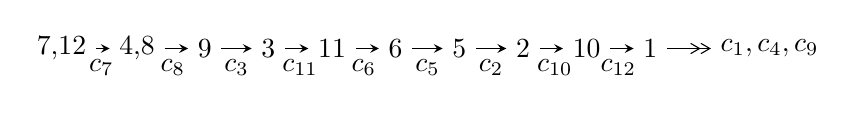
\begin{tikzpicture}[x=23pt, y=7pt]
	% node
	\node (A0) at (-1/8, 0) {7,12};
	\node (A1) at (17/16, 0) {4,8};
	\node (A2) at (17/8, 0) {9};
	\node (A3) at (25/8, 0) {3};
	\node (A4) at (33/8, 0) {11};
	\node (A5) at (41/8, 0) {6};
	\node (A6) at (49/8, 0) {5};
	\node (A7) at (57/8, 0) {2};
	\node (A8) at (65/8, 0) {10};
	\node (A9) at (73/8, 0) {1};
	\node (C1) at (1/2, -1) {$c_{7}$};
	\node (C2) at (13/8, -1) {$c_{8}$};
	\node (C3) at (21/8, -1) {$c_{3}$};
	\node (C4) at (29/8, -1) {$c_{11}$};
	\node (C5) at (37/8, -1) {$c_{6}$};
	\node (C6) at (45/8, -1) {$c_{5}$};
	\node (C7) at (53/8, -1) {$c_{2}$};
	\node (C8) at (61/8, -1) {$c_{10}$};
	\node (C9) at (69/8, -1) {$c_{12}$};
	\node (A10) at (11, 0) {$c_{1},c_{4},c_{9}$};

	% edge
	\draw[->,>=stealth]	
	(A0) edge (A1) (A1) edge (A2) (A2) edge (A3) (A3) edge (A4) (A4) edge (A5) (A5) edge (A6) (A6) edge (A7) (A7) edge (A8) (A8) edge (A9) ;
	\draw[->>,>={angle 60}]	
	(A9) edge (A10);
\end{tikzpicture} \\ 

\end{tabular} \\

\footnotetext{
The image of knot diagram is generated by the software ``\textbf{Draw programme}" developed by Andrew Bartholomew(\url{http://www.layer8.co.uk/maths/draw/index.htm\#Running-draw}), where we modified some parts for our purpose(\url{https://github.com/CATsTAILs/LinksPainter}).
}\phantom \\ \newline 
\centering \textbf{Ideals for irreducible components\footnotemark of $X_{\text{par}}$} 
 
\begin{align*}
I^u_{1}&=\langle 
- u^{77}+41 u^{75}+\cdots+3 u^2+b,\;u^{76}-41 u^{74}+\cdots+a+1,\;u^{78}-2 u^{77}+\cdots+u+1\rangle \\
I^u_{2}&=\langle 
- u^5+2 u^3- u^2+b+1,\;u^5-3 u^3+u^2+a+2 u-2,\;u^6+u^5-3 u^4-2 u^3+2 u^2- u-1\rangle \\
\\
\end{align*}
\raggedright * 2 irreducible components of $\dim_{\mathbb{C}}=0$, with total 84 representations.\\
\footnotetext{All coefficients of polynomials are rational numbers. But the coefficients are sometimes approximated in decimal forms when there is not enough margin.}
\newpage
\renewcommand{\arraystretch}{1}
\centering \section*{I. $I^u_{1}= \langle - u^{77}+41 u^{75}+\cdots+3 u^2+b,\;u^{76}-41 u^{74}+\cdots+a+1,\;u^{78}-2 u^{77}+\cdots+u+1 \rangle$}
\flushleft \textbf{(i) Arc colorings}\\
\begin{tabular}{m{7pt} m{180pt} m{7pt} m{180pt} }
\flushright $a_{7}=$&$\begin{pmatrix}1\\0\end{pmatrix}$ \\
\flushright $a_{12}=$&$\begin{pmatrix}0\\u\end{pmatrix}$ \\
\flushright $a_{4}=$&$\begin{pmatrix}- u^{76}+41 u^{74}+\cdots+u-1\\u^{77}-41 u^{75}+\cdots-3 u^3-3 u^2\end{pmatrix}$ \\
\flushright $a_{8}=$&$\begin{pmatrix}1\\- u^2\end{pmatrix}$ \\
\flushright $a_{9}=$&$\begin{pmatrix}u^{11}-6 u^9+12 u^7-8 u^5+u^3-2 u\\- u^{11}+5 u^9-8 u^7+5 u^5-3 u^3+u\end{pmatrix}$ \\
\flushright $a_{3}=$&$\begin{pmatrix}u^{77}- u^{76}+\cdots+8 u^2-2\\-2 u^{77}+2 u^{76}+\cdots+3 u+2\end{pmatrix}$ \\
\flushright $a_{11}=$&$\begin{pmatrix}- u\\u\end{pmatrix}$ \\
\flushright $a_{6}=$&$\begin{pmatrix}- u^2+1\\u^2\end{pmatrix}$ \\
\flushright $a_{5}=$&$\begin{pmatrix}u^{20}-11 u^{18}+\cdots-3 u^2+1\\- u^{20}+10 u^{18}+\cdots-5 u^4+2 u^2\end{pmatrix}$ \\
\flushright $a_{2}=$&$\begin{pmatrix}u^{77}- u^{76}+\cdots+u-1\\- u^{77}+u^{76}+\cdots+2 u+1\end{pmatrix}$ \\
\flushright $a_{10}=$&$\begin{pmatrix}u^3-2 u\\- u^3+u\end{pmatrix}$ \\
\flushright $a_{1}=$&$\begin{pmatrix}u^7-4 u^5+4 u^3\\- u^7+3 u^5-2 u^3+u\end{pmatrix}$\\&\end{tabular}
\flushleft \textbf{(ii) Obstruction class $= -1$}\\~\\
\flushleft \textbf{(iii) Cusp Shapes $= 8 u^{77}-9 u^{76}+\cdots-18 u+6$}\\~\\
\newpage\renewcommand{\arraystretch}{1}
\flushleft \textbf{(iv) u-Polynomials at the component}\newline \\
\begin{tabular}{m{50pt}|m{274pt}}
Crossings & \hspace{64pt}u-Polynomials at each crossing \\
\hline $$\begin{aligned}c_{1}\end{aligned}$$&$\begin{aligned}
&u^{78}+37 u^{77}+\cdots+114 u+1
\end{aligned}$\\
\hline $$\begin{aligned}c_{2},c_{4}\end{aligned}$$&$\begin{aligned}
&u^{78}-7 u^{77}+\cdots-14 u+1
\end{aligned}$\\
\hline $$\begin{aligned}c_{3},c_{8}\end{aligned}$$&$\begin{aligned}
&u^{78}+u^{77}+\cdots-800 u^2+64
\end{aligned}$\\
\hline $$\begin{aligned}c_{5}\end{aligned}$$&$\begin{aligned}
&u^{78}-2 u^{77}+\cdots-14229 u+4721
\end{aligned}$\\
\hline $$\begin{aligned}c_{6},c_{7},c_{10}\\c_{11}\end{aligned}$$&$\begin{aligned}
&u^{78}+2 u^{77}+\cdots- u+1
\end{aligned}$\\
\hline $$\begin{aligned}c_{9},c_{12}\end{aligned}$$&$\begin{aligned}
&u^{78}+14 u^{77}+\cdots+2121 u+207
\end{aligned}$\\
\hline
\end{tabular}\\~\\
\newpage\renewcommand{\arraystretch}{1}
\flushleft \textbf{(v) Riley Polynomials at the component}\newline \\
\begin{tabular}{m{50pt}|m{274pt}}
Crossings & \hspace{64pt}Riley Polynomials at each crossing \\
\hline $$\begin{aligned}c_{1}\end{aligned}$$&$\begin{aligned}
&y^{78}+15 y^{77}+\cdots-9330 y+1
\end{aligned}$\\
\hline $$\begin{aligned}c_{2},c_{4}\end{aligned}$$&$\begin{aligned}
&y^{78}-37 y^{77}+\cdots-114 y+1
\end{aligned}$\\
\hline $$\begin{aligned}c_{3},c_{8}\end{aligned}$$&$\begin{aligned}
&y^{78}-39 y^{77}+\cdots-102400 y+4096
\end{aligned}$\\
\hline $$\begin{aligned}c_{5}\end{aligned}$$&$\begin{aligned}
&y^{78}-14 y^{77}+\cdots-388528493 y+22287841
\end{aligned}$\\
\hline $$\begin{aligned}c_{6},c_{7},c_{10}\\c_{11}\end{aligned}$$&$\begin{aligned}
&y^{78}-86 y^{77}+\cdots- y+1
\end{aligned}$\\
\hline $$\begin{aligned}c_{9},c_{12}\end{aligned}$$&$\begin{aligned}
&y^{78}+46 y^{77}+\cdots+505791 y+42849
\end{aligned}$\\
\hline
\end{tabular}\\~\\
\newpage\flushleft \textbf{(vi) Complex Volumes and Cusp Shapes}
$$\begin{array}{c|c|c}  
\text{Solutions to }I^u_{1}& \I (\text{vol} + \sqrt{-1}CS) & \text{Cusp shape}\\
 \hline 
\begin{aligned}
u &= -0.599318 + 0.584746 I \\
a &= -1.27127 - 2.26281 I \\
b &= \phantom{-}0.406911 - 0.172691 I\end{aligned}
 & -0.78175 - 12.54030 I & \phantom{-}6.09746 + 10.28095 I \\ \hline\begin{aligned}
u &= -0.599318 - 0.584746 I \\
a &= -1.27127 + 2.26281 I \\
b &= \phantom{-}0.406911 + 0.172691 I\end{aligned}
 & -0.78175 + 12.54030 I & \phantom{-}6.09746 - 10.28095 I \\ \hline\begin{aligned}
u &= -0.599850 + 0.564094 I \\
a &= \phantom{-}1.27636 + 2.11108 I \\
b &= -0.278346 + 0.277845 I\end{aligned}
 & \phantom{-}1.55983 - 6.97653 I & \phantom{-}9.24019 + 6.64171 I \\ \hline\begin{aligned}
u &= -0.599850 - 0.564094 I \\
a &= \phantom{-}1.27636 - 2.11108 I \\
b &= -0.278346 - 0.277845 I\end{aligned}
 & \phantom{-}1.55983 + 6.97653 I & \phantom{-}9.24019 - 6.64171 I \\ \hline\begin{aligned}
u &= \phantom{-}0.802841 + 0.168457 I \\
a &= -2.26912 + 0.63093 I \\
b &= \phantom{-}0.357877 - 0.320430 I\end{aligned}
 & \phantom{-}3.97087 + 7.20217 I & \phantom{-}11.97302 - 7.33202 I \\ \hline\begin{aligned}
u &= \phantom{-}0.802841 - 0.168457 I \\
a &= -2.26912 - 0.63093 I \\
b &= \phantom{-}0.357877 + 0.320430 I\end{aligned}
 & \phantom{-}3.97087 - 7.20217 I & \phantom{-}11.97302 + 7.33202 I \\ \hline\begin{aligned}
u &= \phantom{-}0.805439 + 0.096765 I \\
a &= \phantom{-}2.36172 - 0.39872 I \\
b &= -0.359916 + 0.190669 I\end{aligned}
 & \phantom{-}5.68267 + 1.74998 I & \phantom{-}15.1419 - 1.8440 I \\ \hline\begin{aligned}
u &= \phantom{-}0.805439 - 0.096765 I \\
a &= \phantom{-}2.36172 + 0.39872 I \\
b &= -0.359916 - 0.190669 I\end{aligned}
 & \phantom{-}5.68267 - 1.74998 I & \phantom{-}15.1419 + 1.8440 I \\ \hline\begin{aligned}
u &= \phantom{-}0.576717 + 0.560895 I \\
a &= \phantom{-}1.345380 - 0.149355 I \\
b &= -0.580995 + 0.149181 I\end{aligned}
 & -3.14364 + 6.35997 I & \phantom{-}4.39196 - 7.72214 I \\ \hline\begin{aligned}
u &= \phantom{-}0.576717 - 0.560895 I \\
a &= \phantom{-}1.345380 + 0.149355 I \\
b &= -0.580995 - 0.149181 I\end{aligned}
 & -3.14364 - 6.35997 I & \phantom{-}4.39196 + 7.72214 I\\
 \hline 
 \end{array}$$\newpage$$\begin{array}{c|c|c}  
\text{Solutions to }I^u_{1}& \I (\text{vol} + \sqrt{-1}CS) & \text{Cusp shape}\\
 \hline 
\begin{aligned}
u &= \phantom{-}0.520959 + 0.606760 I \\
a &= \phantom{-}0.872173 + 0.421611 I \\
b &= -0.423627 - 0.168563 I\end{aligned}
 & -4.39476 + 0.68401 I & \phantom{-}5.05755 + 1.70512 I \\ \hline\begin{aligned}
u &= \phantom{-}0.520959 - 0.606760 I \\
a &= \phantom{-}0.872173 - 0.421611 I \\
b &= -0.423627 + 0.168563 I\end{aligned}
 & -4.39476 - 0.68401 I & \phantom{-}5.05755 - 1.70512 I \\ \hline\begin{aligned}
u &= -0.558404 + 0.553380 I \\
a &= -1.70602 - 1.99005 I \\
b &= \phantom{-}0.351192 - 0.673255 I\end{aligned}
 & -4.00256 - 3.82936 I & \phantom{-}4.97815 + 7.00642 I \\ \hline\begin{aligned}
u &= -0.558404 - 0.553380 I \\
a &= -1.70602 + 1.99005 I \\
b &= \phantom{-}0.351192 + 0.673255 I\end{aligned}
 & -4.00256 + 3.82936 I & \phantom{-}4.97815 - 7.00642 I \\ \hline\begin{aligned}
u &= -0.616947 + 0.471605 I \\
a &= \phantom{-}0.92409 + 1.52711 I \\
b &= \phantom{-}0.200273 + 0.380587 I\end{aligned}
 & \phantom{-}3.37693 - 3.48998 I & \phantom{-}11.29099 + 6.45217 I \\ \hline\begin{aligned}
u &= -0.616947 - 0.471605 I \\
a &= \phantom{-}0.92409 - 1.52711 I \\
b &= \phantom{-}0.200273 - 0.380587 I\end{aligned}
 & \phantom{-}3.37693 + 3.48998 I & \phantom{-}11.29099 - 6.45217 I \\ \hline\begin{aligned}
u &= \phantom{-}0.463830 + 0.615489 I \\
a &= -0.400498 - 0.952066 I \\
b &= \phantom{-}0.193565 + 0.455914 I\end{aligned}
 & -4.56309 + 3.47022 I & \phantom{-}4.07696 - 8.07073 I \\ \hline\begin{aligned}
u &= \phantom{-}0.463830 - 0.615489 I \\
a &= -0.400498 + 0.952066 I \\
b &= \phantom{-}0.193565 - 0.455914 I\end{aligned}
 & -4.56309 - 3.47022 I & \phantom{-}4.07696 + 8.07073 I \\ \hline\begin{aligned}
u &= -0.640817 + 0.405593 I \\
a &= -0.62536 - 1.32558 I \\
b &= -0.339137 - 0.372642 I\end{aligned}
 & \phantom{-}2.45756 + 1.82034 I & \phantom{-}10.30646 + 0.66101 I \\ \hline\begin{aligned}
u &= -0.640817 - 0.405593 I \\
a &= -0.62536 + 1.32558 I \\
b &= -0.339137 + 0.372642 I\end{aligned}
 & \phantom{-}2.45756 - 1.82034 I & \phantom{-}10.30646 - 0.66101 I\\
 \hline 
 \end{array}$$\newpage$$\begin{array}{c|c|c}  
\text{Solutions to }I^u_{1}& \I (\text{vol} + \sqrt{-1}CS) & \text{Cusp shape}\\
 \hline 
\begin{aligned}
u &= \phantom{-}0.541710 + 0.519985 I \\
a &= -1.108600 + 0.518660 I \\
b &= \phantom{-}0.443108 - 0.259777 I\end{aligned}
 & -1.72128 + 2.09820 I & \phantom{-}6.19910 - 2.97697 I \\ \hline\begin{aligned}
u &= \phantom{-}0.541710 - 0.519985 I \\
a &= -1.108600 - 0.518660 I \\
b &= \phantom{-}0.443108 + 0.259777 I\end{aligned}
 & -1.72128 - 2.09820 I & \phantom{-}6.19910 + 2.97697 I \\ \hline\begin{aligned}
u &= -0.364533 + 0.621473 I \\
a &= -0.308159 - 0.767887 I \\
b &= \phantom{-}1.44780 + 0.32955 I\end{aligned}
 & -1.47143 + 8.43896 I & \phantom{-}4.23505 - 4.36846 I \\ \hline\begin{aligned}
u &= -0.364533 - 0.621473 I \\
a &= -0.308159 + 0.767887 I \\
b &= \phantom{-}1.44780 - 0.32955 I\end{aligned}
 & -1.47143 - 8.43896 I & \phantom{-}4.23505 + 4.36846 I \\ \hline\begin{aligned}
u &= -0.710687 + 0.078003 I \\
a &= -0.060076 - 0.763572 I \\
b &= -0.130706 - 0.534050 I\end{aligned}
 & \phantom{-}0.94742 - 1.90115 I & \phantom{-}11.49371 + 4.32216 I \\ \hline\begin{aligned}
u &= -0.710687 - 0.078003 I \\
a &= -0.060076 + 0.763572 I \\
b &= -0.130706 + 0.534050 I\end{aligned}
 & \phantom{-}0.94742 + 1.90115 I & \phantom{-}11.49371 - 4.32216 I \\ \hline\begin{aligned}
u &= -0.408883 + 0.562647 I \\
a &= \phantom{-}0.668680 - 0.785887 I \\
b &= \phantom{-}1.29216 + 0.60980 I\end{aligned}
 & -4.44211 - 0.01380 I & \phantom{-}2.92184 - 0.24930 I \\ \hline\begin{aligned}
u &= -0.408883 - 0.562647 I \\
a &= \phantom{-}0.668680 + 0.785887 I \\
b &= \phantom{-}1.29216 - 0.60980 I\end{aligned}
 & -4.44211 + 0.01380 I & \phantom{-}2.92184 + 0.24930 I \\ \hline\begin{aligned}
u &= \phantom{-}0.383552 + 0.577713 I \\
a &= \phantom{-}0.12013 - 1.41029 I \\
b &= -0.127003 + 0.649722 I\end{aligned}
 & -3.70836 - 2.45187 I & \phantom{-}2.28902 + 1.10557 I \\ \hline\begin{aligned}
u &= \phantom{-}0.383552 - 0.577713 I \\
a &= \phantom{-}0.12013 + 1.41029 I \\
b &= -0.127003 - 0.649722 I\end{aligned}
 & -3.70836 + 2.45187 I & \phantom{-}2.28902 - 1.10557 I\\
 \hline 
 \end{array}$$\newpage$$\begin{array}{c|c|c}  
\text{Solutions to }I^u_{1}& \I (\text{vol} + \sqrt{-1}CS) & \text{Cusp shape}\\
 \hline 
\begin{aligned}
u &= -0.350709 + 0.593744 I \\
a &= \phantom{-}0.107351 + 0.504864 I \\
b &= -1.343700 - 0.316084 I\end{aligned}
 & \phantom{-}0.83358 + 3.01735 I & \phantom{-}7.25837 - 0.49247 I \\ \hline\begin{aligned}
u &= -0.350709 - 0.593744 I \\
a &= \phantom{-}0.107351 - 0.504864 I \\
b &= -1.343700 + 0.316084 I\end{aligned}
 & \phantom{-}0.83358 - 3.01735 I & \phantom{-}7.25837 + 0.49247 I \\ \hline\begin{aligned}
u &= \phantom{-}0.442910 + 0.518440 I \\
a &= -0.521192 + 1.076400 I \\
b &= \phantom{-}0.241180 - 0.446445 I\end{aligned}
 & -2.02036 + 1.50879 I & \phantom{-}4.97629 - 5.09309 I \\ \hline\begin{aligned}
u &= \phantom{-}0.442910 - 0.518440 I \\
a &= -0.521192 - 1.076400 I \\
b &= \phantom{-}0.241180 + 0.446445 I\end{aligned}
 & -2.02036 - 1.50879 I & \phantom{-}4.97629 + 5.09309 I \\ \hline\begin{aligned}
u &= \phantom{-}0.645827\phantom{ +0.000000I} \\
a &= -3.49684\phantom{ +0.000000I} \\
b &= \phantom{-}0.752757\phantom{ +0.000000I}\end{aligned}
 & -0.308788\phantom{ +0.000000I} & \phantom{-}16.2550\phantom{ +0.000000I} \\ \hline\begin{aligned}
u &= \phantom{-}1.42939 + 0.12884 I \\
a &= -0.715223 - 0.199859 I \\
b &= \phantom{-}0.242567 + 1.308940 I\end{aligned}
 & \phantom{-}4.19828 - 5.82838 I & \phantom{-0.000000 } 0 \\ \hline\begin{aligned}
u &= \phantom{-}1.42939 - 0.12884 I \\
a &= -0.715223 + 0.199859 I \\
b &= \phantom{-}0.242567 - 1.308940 I\end{aligned}
 & \phantom{-}4.19828 + 5.82838 I & \phantom{-0.000000 } 0 \\ \hline\begin{aligned}
u &= \phantom{-}1.44778 + 0.09666 I \\
a &= \phantom{-}0.890808 + 0.121968 I \\
b &= -0.777252 - 0.958438 I\end{aligned}
 & \phantom{-}6.48020 - 0.70488 I & \phantom{-0.000000 } 0 \\ \hline\begin{aligned}
u &= \phantom{-}1.44778 - 0.09666 I \\
a &= \phantom{-}0.890808 - 0.121968 I \\
b &= -0.777252 + 0.958438 I\end{aligned}
 & \phantom{-}6.48020 + 0.70488 I & \phantom{-0.000000 } 0 \\ \hline\begin{aligned}
u &= -0.219534 + 0.501040 I \\
a &= \phantom{-}0.048525 - 0.591352 I \\
b &= -0.992560 + 0.039651 I\end{aligned}
 & \phantom{-}2.27210 + 0.14195 I & \phantom{-}7.85107 + 0.40000 I\\
 \hline 
 \end{array}$$\newpage$$\begin{array}{c|c|c}  
\text{Solutions to }I^u_{1}& \I (\text{vol} + \sqrt{-1}CS) & \text{Cusp shape}\\
 \hline 
\begin{aligned}
u &= -0.219534 - 0.501040 I \\
a &= \phantom{-}0.048525 + 0.591352 I \\
b &= -0.992560 - 0.039651 I\end{aligned}
 & \phantom{-}2.27210 - 0.14195 I & \phantom{-}7.85107 - 0.40000 I \\ \hline\begin{aligned}
u &= -0.128219 + 0.511830 I \\
a &= -0.235116 + 0.964407 I \\
b &= \phantom{-}0.956059 - 0.264958 I\end{aligned}
 & \phantom{-}0.94305 - 4.90661 I & \phantom{-}4.88398 + 5.62400 I \\ \hline\begin{aligned}
u &= -0.128219 - 0.511830 I \\
a &= -0.235116 - 0.964407 I \\
b &= \phantom{-}0.956059 + 0.264958 I\end{aligned}
 & \phantom{-}0.94305 + 4.90661 I & \phantom{-}4.88398 - 5.62400 I \\ \hline\begin{aligned}
u &= -1.47226 + 0.12075 I \\
a &= -0.646554 - 0.603418 I \\
b &= \phantom{-}1.07448 + 1.96891 I\end{aligned}
 & \phantom{-}2.26225 + 0.10898 I & \phantom{-0.000000 } 0 \\ \hline\begin{aligned}
u &= -1.47226 - 0.12075 I \\
a &= -0.646554 + 0.603418 I \\
b &= \phantom{-}1.07448 - 1.96891 I\end{aligned}
 & \phantom{-}2.26225 - 0.10898 I & \phantom{-0.000000 } 0 \\ \hline\begin{aligned}
u &= \phantom{-}1.48782 + 0.13055 I \\
a &= -1.266260 - 0.496751 I \\
b &= \phantom{-}1.79248 + 2.09730 I\end{aligned}
 & \phantom{-}1.73920 + 2.36195 I & \phantom{-0.000000 } 0 \\ \hline\begin{aligned}
u &= \phantom{-}1.48782 - 0.13055 I \\
a &= -1.266260 + 0.496751 I \\
b &= \phantom{-}1.79248 - 2.09730 I\end{aligned}
 & \phantom{-}1.73920 - 2.36195 I & \phantom{-0.000000 } 0 \\ \hline\begin{aligned}
u &= -1.49302 + 0.17302 I \\
a &= -0.365143 - 0.576564 I \\
b &= \phantom{-}0.27170 + 1.51342 I\end{aligned}
 & \phantom{-}1.82198 - 6.26698 I & \phantom{-0.000000 } 0 \\ \hline\begin{aligned}
u &= -1.49302 - 0.17302 I \\
a &= -0.365143 + 0.576564 I \\
b &= \phantom{-}0.27170 - 1.51342 I\end{aligned}
 & \phantom{-}1.82198 + 6.26698 I & \phantom{-0.000000 } 0 \\ \hline\begin{aligned}
u &= \phantom{-}1.51505\phantom{ +0.000000I} \\
a &= \phantom{-}0.596370\phantom{ +0.000000I} \\
b &= -0.787410\phantom{ +0.000000I}\end{aligned}
 & \phantom{-}7.16001\phantom{ +0.000000I} & \phantom{-0.000000 } 0\\
 \hline 
 \end{array}$$\newpage$$\begin{array}{c|c|c}  
\text{Solutions to }I^u_{1}& \I (\text{vol} + \sqrt{-1}CS) & \text{Cusp shape}\\
 \hline 
\begin{aligned}
u &= -1.51198 + 0.13240 I \\
a &= \phantom{-}0.718360 + 0.295013 I \\
b &= -1.39217 - 1.12726 I\end{aligned}
 & \phantom{-}4.46397 - 3.74584 I & \phantom{-0.000000 } 0 \\ \hline\begin{aligned}
u &= -1.51198 - 0.13240 I \\
a &= \phantom{-}0.718360 - 0.295013 I \\
b &= -1.39217 + 1.12726 I\end{aligned}
 & \phantom{-}4.46397 + 3.74584 I & \phantom{-0.000000 } 0 \\ \hline\begin{aligned}
u &= -1.52531 + 0.18019 I \\
a &= -0.095957 + 0.602649 I \\
b &= \phantom{-}0.632159 - 1.131610 I\end{aligned}
 & \phantom{-}2.35354 - 3.51433 I & \phantom{-0.000000 } 0 \\ \hline\begin{aligned}
u &= -1.52531 - 0.18019 I \\
a &= -0.095957 - 0.602649 I \\
b &= \phantom{-}0.632159 + 1.131610 I\end{aligned}
 & \phantom{-}2.35354 + 3.51433 I & \phantom{-0.000000 } 0 \\ \hline\begin{aligned}
u &= -1.54784 + 0.15010 I \\
a &= \phantom{-}0.800421 - 0.348125 I \\
b &= -1.84286 + 0.24135 I\end{aligned}
 & \phantom{-}5.27378 - 4.50564 I & \phantom{-0.000000 } 0 \\ \hline\begin{aligned}
u &= -1.54784 - 0.15010 I \\
a &= \phantom{-}0.800421 + 0.348125 I \\
b &= -1.84286 - 0.24135 I\end{aligned}
 & \phantom{-}5.27378 + 4.50564 I & \phantom{-0.000000 } 0 \\ \hline\begin{aligned}
u &= \phantom{-}1.54914 + 0.16225 I \\
a &= \phantom{-}2.40899 - 1.35253 I \\
b &= -5.46000 + 2.34055 I\end{aligned}
 & \phantom{-}3.02625 + 6.41510 I & \phantom{-0.000000 } 0 \\ \hline\begin{aligned}
u &= \phantom{-}1.54914 - 0.16225 I \\
a &= \phantom{-}2.40899 + 1.35253 I \\
b &= -5.46000 - 2.34055 I\end{aligned}
 & \phantom{-}3.02625 - 6.41510 I & \phantom{-0.000000 } 0 \\ \hline\begin{aligned}
u &= -1.55516 + 0.16682 I \\
a &= -0.698192 + 0.656632 I \\
b &= \phantom{-}1.77866 - 0.87693 I\end{aligned}
 & \phantom{-}3.96996 - 9.00544 I & \phantom{-0.000000 } 0 \\ \hline\begin{aligned}
u &= -1.55516 - 0.16682 I \\
a &= -0.698192 - 0.656632 I \\
b &= \phantom{-}1.77866 + 0.87693 I\end{aligned}
 & \phantom{-}3.96996 + 9.00544 I & \phantom{-0.000000 } 0\\
 \hline 
 \end{array}$$\newpage$$\begin{array}{c|c|c}  
\text{Solutions to }I^u_{1}& \I (\text{vol} + \sqrt{-1}CS) & \text{Cusp shape}\\
 \hline 
\begin{aligned}
u &= \phantom{-}1.56285 + 0.17763 I \\
a &= \phantom{-}2.12209 - 1.39087 I \\
b &= -4.66821 + 2.86534 I\end{aligned}
 & \phantom{-}6.4302 + 15.3326 I & \phantom{-0.000000 } 0 \\ \hline\begin{aligned}
u &= \phantom{-}1.56285 - 0.17763 I \\
a &= \phantom{-}2.12209 + 1.39087 I \\
b &= -4.66821 - 2.86534 I\end{aligned}
 & \phantom{-}6.4302 - 15.3326 I & \phantom{-0.000000 } 0 \\ \hline\begin{aligned}
u &= \phantom{-}1.56376 + 0.16947 I \\
a &= -2.16477 + 1.35365 I \\
b &= \phantom{-}4.71147 - 2.63450 I\end{aligned}
 & \phantom{-}8.79025 + 9.66014 I & \phantom{-0.000000 } 0 \\ \hline\begin{aligned}
u &= \phantom{-}1.56376 - 0.16947 I \\
a &= -2.16477 - 1.35365 I \\
b &= \phantom{-}4.71147 + 2.63450 I\end{aligned}
 & \phantom{-}8.79025 - 9.66014 I & \phantom{-0.000000 } 0 \\ \hline\begin{aligned}
u &= -1.57499\phantom{ +0.000000I} \\
a &= \phantom{-}3.21218\phantom{ +0.000000I} \\
b &= -7.08625\phantom{ +0.000000I}\end{aligned}
 & \phantom{-}7.27373\phantom{ +0.000000I} & \phantom{-0.000000 } 0 \\ \hline\begin{aligned}
u &= \phantom{-}1.57066 + 0.11845 I \\
a &= \phantom{-}1.72662 - 1.03255 I \\
b &= -3.35704 + 1.54534 I\end{aligned}
 & \phantom{-}9.89816 + 0.10218 I & \phantom{-0.000000 } 0 \\ \hline\begin{aligned}
u &= \phantom{-}1.57066 - 0.11845 I \\
a &= \phantom{-}1.72662 + 1.03255 I \\
b &= -3.35704 - 1.54534 I\end{aligned}
 & \phantom{-}9.89816 - 0.10218 I & \phantom{-0.000000 } 0 \\ \hline\begin{aligned}
u &= \phantom{-}1.56925 + 0.13763 I \\
a &= -1.97809 + 1.10921 I \\
b &= \phantom{-}4.00616 - 1.77495 I\end{aligned}
 & \phantom{-}10.73110 + 5.71945 I & \phantom{-0.000000 } 0 \\ \hline\begin{aligned}
u &= \phantom{-}1.56925 - 0.13763 I \\
a &= -1.97809 - 1.10921 I \\
b &= \phantom{-}4.00616 + 1.77495 I\end{aligned}
 & \phantom{-}10.73110 - 5.71945 I & \phantom{-0.000000 } 0 \\ \hline\begin{aligned}
u &= -0.417322\phantom{ +0.000000I} \\
a &= -0.507402\phantom{ +0.000000I} \\
b &= -0.228914\phantom{ +0.000000I}\end{aligned}
 & \phantom{-}0.609628\phantom{ +0.000000I} & \phantom{-}16.4390\phantom{ +0.000000I}\\
 \hline 
 \end{array}$$\newpage$$\begin{array}{c|c|c}  
\text{Solutions to }I^u_{1}& \I (\text{vol} + \sqrt{-1}CS) & \text{Cusp shape}\\
 \hline 
\begin{aligned}
u &= \phantom{-}1.58333 + 0.01332 I \\
a &= \phantom{-}0.212622 - 1.085020 I \\
b &= -0.36367 + 1.69619 I\end{aligned}
 & \phantom{-}8.73171 + 2.18417 I & \phantom{-0.000000 } 0 \\ \hline\begin{aligned}
u &= \phantom{-}1.58333 - 0.01332 I \\
a &= \phantom{-}0.212622 + 1.085020 I \\
b &= -0.36367 - 1.69619 I\end{aligned}
 & \phantom{-}8.73171 - 2.18417 I & \phantom{-0.000000 } 0 \\ \hline\begin{aligned}
u &= -1.60086 + 0.01874 I \\
a &= -2.81392 - 0.07195 I \\
b &= \phantom{-}5.91931 + 0.33569 I\end{aligned}
 & \phantom{-}13.82740 - 2.12508 I & \phantom{-0.000000 } 0 \\ \hline\begin{aligned}
u &= -1.60086 - 0.01874 I \\
a &= -2.81392 + 0.07195 I \\
b &= \phantom{-}5.91931 - 0.33569 I\end{aligned}
 & \phantom{-}13.82740 + 2.12508 I & \phantom{-0.000000 } 0 \\ \hline\begin{aligned}
u &= -1.60129 + 0.03305 I \\
a &= \phantom{-}2.69061 + 0.07587 I \\
b &= -5.63287 - 0.46743 I\end{aligned}
 & \phantom{-}12.1159 - 7.8628 I & \phantom{-0.000000 } 0 \\ \hline\begin{aligned}
u &= -1.60129 - 0.03305 I \\
a &= \phantom{-}2.69061 - 0.07587 I \\
b &= -5.63287 + 0.46743 I\end{aligned}
 & \phantom{-}12.1159 + 7.8628 I & \phantom{-0.000000 } 0 \\ \hline\begin{aligned}
u &= \phantom{-}0.119394 + 0.283485 I \\
a &= \phantom{-}0.05243 + 2.15878 I \\
b &= \phantom{-}0.425883 - 0.450283 I\end{aligned}
 & -1.64524 + 0.68396 I & -1.89365 - 2.07297 I \\ \hline\begin{aligned}
u &= \phantom{-}0.119394 - 0.283485 I \\
a &= \phantom{-}0.05243 - 2.15878 I \\
b &= \phantom{-}0.425883 + 0.450283 I\end{aligned}
 & -1.64524 - 0.68396 I & -1.89365 + 2.07297 I\\
 \hline 
 \end{array}$$\newpage\newpage\renewcommand{\arraystretch}{1}
\centering \section*{II. $I^u_{2}= \langle - u^5+2 u^3- u^2+b+1,\;u^5-3 u^3+u^2+a+2 u-2,\;u^6+u^5-3 u^4-2 u^3+2 u^2- u-1 \rangle$}
\flushleft \textbf{(i) Arc colorings}\\
\begin{tabular}{m{7pt} m{180pt} m{7pt} m{180pt} }
\flushright $a_{7}=$&$\begin{pmatrix}1\\0\end{pmatrix}$ \\
\flushright $a_{12}=$&$\begin{pmatrix}0\\u\end{pmatrix}$ \\
\flushright $a_{4}=$&$\begin{pmatrix}- u^5+3 u^3- u^2-2 u+2\\u^5-2 u^3+u^2-1\end{pmatrix}$ \\
\flushright $a_{8}=$&$\begin{pmatrix}1\\- u^2\end{pmatrix}$ \\
\flushright $a_{9}=$&$\begin{pmatrix}1\\- u^2\end{pmatrix}$ \\
\flushright $a_{3}=$&$\begin{pmatrix}- u^5+3 u^3- u^2-2 u+2\\u^5-2 u^3+u^2-1\end{pmatrix}$ \\
\flushright $a_{11}=$&$\begin{pmatrix}- u\\u\end{pmatrix}$ \\
\flushright $a_{6}=$&$\begin{pmatrix}- u^2+1\\u^2\end{pmatrix}$ \\
\flushright $a_{5}=$&$\begin{pmatrix}u^4-3 u^2+1\\u^5- u^4-2 u^3+3 u^2- u-1\end{pmatrix}$ \\
\flushright $a_{2}=$&$\begin{pmatrix}- u^5- u^4+3 u^3+2 u^2-2 u+1\\u^4-2 u^2+u\end{pmatrix}$ \\
\flushright $a_{10}=$&$\begin{pmatrix}u^3-2 u\\- u^3+u\end{pmatrix}$ \\
\flushright $a_{1}=$&$\begin{pmatrix}- u^4+3 u^2-1\\- u^5+u^4+2 u^3-3 u^2+u+1\end{pmatrix}$\\&\end{tabular}
\flushleft \textbf{(ii) Obstruction class $= 1$}\\~\\
\flushleft \textbf{(iii) Cusp Shapes $= 3 u^5+u^4-6 u^3- u^2-2 u+2$}\\~\\
\newpage\renewcommand{\arraystretch}{1}
\flushleft \textbf{(iv) u-Polynomials at the component}\newline \\
\begin{tabular}{m{50pt}|m{274pt}}
Crossings & \hspace{64pt}u-Polynomials at each crossing \\
\hline $$\begin{aligned}c_{1},c_{2}\end{aligned}$$&$\begin{aligned}
&(u-1)^6
\end{aligned}$\\
\hline $$\begin{aligned}c_{3},c_{8}\end{aligned}$$&$\begin{aligned}
&u^6
\end{aligned}$\\
\hline $$\begin{aligned}c_{4}\end{aligned}$$&$\begin{aligned}
&(u+1)^6
\end{aligned}$\\
\hline $$\begin{aligned}c_{5},c_{9}\end{aligned}$$&$\begin{aligned}
&u^6- u^5+3 u^4-2 u^3+2 u^2- u-1
\end{aligned}$\\
\hline $$\begin{aligned}c_{6},c_{7}\end{aligned}$$&$\begin{aligned}
&u^6+u^5-3 u^4-2 u^3+2 u^2- u-1
\end{aligned}$\\
\hline $$\begin{aligned}c_{10},c_{11}\end{aligned}$$&$\begin{aligned}
&u^6- u^5-3 u^4+2 u^3+2 u^2+u-1
\end{aligned}$\\
\hline $$\begin{aligned}c_{12}\end{aligned}$$&$\begin{aligned}
&u^6+u^5+3 u^4+2 u^3+2 u^2+u-1
\end{aligned}$\\
\hline
\end{tabular}\\~\\
\newpage\renewcommand{\arraystretch}{1}
\flushleft \textbf{(v) Riley Polynomials at the component}\newline \\
\begin{tabular}{m{50pt}|m{274pt}}
Crossings & \hspace{64pt}Riley Polynomials at each crossing \\
\hline $$\begin{aligned}c_{1},c_{2},c_{4}\end{aligned}$$&$\begin{aligned}
&(y-1)^6
\end{aligned}$\\
\hline $$\begin{aligned}c_{3},c_{8}\end{aligned}$$&$\begin{aligned}
&y^6
\end{aligned}$\\
\hline $$\begin{aligned}c_{5},c_{9},c_{12}\end{aligned}$$&$\begin{aligned}
&y^6+5 y^5+9 y^4+4 y^3-6 y^2-5 y+1
\end{aligned}$\\
\hline $$\begin{aligned}c_{6},c_{7},c_{10}\\c_{11}\end{aligned}$$&$\begin{aligned}
&y^6-7 y^5+17 y^4-16 y^3+6 y^2-5 y+1
\end{aligned}$\\
\hline
\end{tabular}\\~\\
\newpage\flushleft \textbf{(vi) Complex Volumes and Cusp Shapes}
$$\begin{array}{c|c|c}  
\text{Solutions to }I^u_{2}& \I (\text{vol} + \sqrt{-1}CS) & \text{Cusp shape}\\
 \hline 
\begin{aligned}
u &= \phantom{-}0.493180 + 0.575288 I \\
a &= \phantom{-}0.089969 - 0.799962 I \\
b &= -0.446039 - 0.121233 I\end{aligned}
 & -4.60518 + 1.97241 I & \phantom{-}2.71215 - 3.88360 I \\ \hline\begin{aligned}
u &= \phantom{-}0.493180 - 0.575288 I \\
a &= \phantom{-}0.089969 + 0.799962 I \\
b &= -0.446039 + 0.121233 I\end{aligned}
 & -4.60518 - 1.97241 I & \phantom{-}2.71215 + 3.88360 I \\ \hline\begin{aligned}
u &= -0.483672\phantom{ +0.000000I} \\
a &= \phantom{-}2.42043\phantom{ +0.000000I} \\
b &= -0.566232\phantom{ +0.000000I}\end{aligned}
 & -0.906083\phantom{ +0.000000I} & \phantom{-}3.38760\phantom{ +0.000000I} \\ \hline\begin{aligned}
u &= -1.52087 + 0.16310 I \\
a &= -0.227586 - 0.710576 I \\
b &= \phantom{-}0.87287 + 1.51178 I\end{aligned}
 & \phantom{-}2.05064 - 4.59213 I & \phantom{-}6.49628 + 3.92496 I \\ \hline\begin{aligned}
u &= -1.52087 - 0.16310 I \\
a &= -0.227586 + 0.710576 I \\
b &= \phantom{-}0.87287 - 1.51178 I\end{aligned}
 & \phantom{-}2.05064 + 4.59213 I & \phantom{-}6.49628 - 3.92496 I \\ \hline\begin{aligned}
u &= \phantom{-}1.53904\phantom{ +0.000000I} \\
a &= -1.14519\phantom{ +0.000000I} \\
b &= \phantom{-}2.71257\phantom{ +0.000000I}\end{aligned}
 & \phantom{-}6.01515\phantom{ +0.000000I} & \phantom{-}6.19550\phantom{ +0.000000I}\\
 \hline 
 \end{array}$$\newpage
\newpage\renewcommand{\arraystretch}{1}
\centering \section*{ III. u-Polynomials}
\begin{tabular}{m{50pt}|m{274pt}}
Crossings & \hspace{64pt}u-Polynomials at each crossing \\
\hline $$\begin{aligned}c_{1}\end{aligned}$$&$\begin{aligned}
&((u-1)^6)(u^{78}+37 u^{77}+\cdots+114 u+1)
\end{aligned}$\\
\hline $$\begin{aligned}c_{2}\end{aligned}$$&$\begin{aligned}
&((u-1)^6)(u^{78}-7 u^{77}+\cdots-14 u+1)
\end{aligned}$\\
\hline $$\begin{aligned}c_{3},c_{8}\end{aligned}$$&$\begin{aligned}
&u^6(u^{78}+u^{77}+\cdots-800 u^2+64)
\end{aligned}$\\
\hline $$\begin{aligned}c_{4}\end{aligned}$$&$\begin{aligned}
&((u+1)^6)(u^{78}-7 u^{77}+\cdots-14 u+1)
\end{aligned}$\\
\hline $$\begin{aligned}c_{5}\end{aligned}$$&$\begin{aligned}
&(u^6- u^5+3 u^4-2 u^3+2 u^2- u-1)(u^{78}-2 u^{77}+\cdots-14229 u+4721)
\end{aligned}$\\
\hline $$\begin{aligned}c_{6},c_{7}\end{aligned}$$&$\begin{aligned}
&(u^6+u^5-3 u^4-2 u^3+2 u^2- u-1)(u^{78}+2 u^{77}+\cdots- u+1)
\end{aligned}$\\
\hline $$\begin{aligned}c_{9}\end{aligned}$$&$\begin{aligned}
&(u^6- u^5+3 u^4-2 u^3+2 u^2- u-1)(u^{78}+14 u^{77}+\cdots+2121 u+207)
\end{aligned}$\\
\hline $$\begin{aligned}c_{10},c_{11}\end{aligned}$$&$\begin{aligned}
&(u^6- u^5-3 u^4+2 u^3+2 u^2+u-1)(u^{78}+2 u^{77}+\cdots- u+1)
\end{aligned}$\\
\hline $$\begin{aligned}c_{12}\end{aligned}$$&$\begin{aligned}
&(u^6+u^5+3 u^4+2 u^3+2 u^2+u-1)(u^{78}+14 u^{77}+\cdots+2121 u+207)
\end{aligned}$\\
\hline
\end{tabular}\newpage\renewcommand{\arraystretch}{1}
\centering \section*{ IV. Riley Polynomials}
\begin{tabular}{m{50pt}|m{274pt}}
Crossings & \hspace{64pt}Riley Polynomials at each crossing \\
\hline $$\begin{aligned}c_{1}\end{aligned}$$&$\begin{aligned}
&((y-1)^6)(y^{78}+15 y^{77}+\cdots-9330 y+1)
\end{aligned}$\\
\hline $$\begin{aligned}c_{2},c_{4}\end{aligned}$$&$\begin{aligned}
&((y-1)^6)(y^{78}-37 y^{77}+\cdots-114 y+1)
\end{aligned}$\\
\hline $$\begin{aligned}c_{3},c_{8}\end{aligned}$$&$\begin{aligned}
&y^6(y^{78}-39 y^{77}+\cdots-102400 y+4096)
\end{aligned}$\\
\hline $$\begin{aligned}c_{5}\end{aligned}$$&$\begin{aligned}
&(y^6+5 y^5+9 y^4+4 y^3-6 y^2-5 y+1)\\
&\cdot(y^{78}-14 y^{77}+\cdots-388528493 y+22287841)
\end{aligned}$\\
\hline $$\begin{aligned}c_{6},c_{7},c_{10}\\c_{11}\end{aligned}$$&$\begin{aligned}
&(y^6-7 y^5+\cdots-5 y+1)(y^{78}-86 y^{77}+\cdots- y+1)
\end{aligned}$\\
\hline $$\begin{aligned}c_{9},c_{12}\end{aligned}$$&$\begin{aligned}
&(y^6+5 y^5+9 y^4+4 y^3-6 y^2-5 y+1)\\
&\cdot(y^{78}+46 y^{77}+\cdots+505791 y+42849)
\end{aligned}$\\
\hline
\end{tabular}
\vskip 2pc
\end{document}